\begin{tikzpicture}[
    font=\sffamily,
    x=1cm,y=1cm,
    flowbox/.style={draw=black!55, line width=0.45pt, rounded corners=2pt, fill=white, align=center, inner sep=3pt},
    groupbox/.style={flowbox, fill=blue!3},
    childbox/.style={flowbox, fill=white, minimum height=0.42cm},
    metricbox/.style={flowbox, fill=green!6, minimum height=0.44cm},
    arrow/.style={-{Latex[length=2.2mm]}, draw=black!65, line width=0.55pt},
    title/.style={font=\bfseries\small, text=black!85},
    tiny/.style={font=\fontsize{6.5}{7.5}\selectfont, text=black!75}
]
\node[groupbox, minimum width=3.0cm, minimum height=4.75cm] (data) at (0,0) {};
\node[title] at ([yshift=-0.28cm]data.north) {VQA data};
\node[tiny, align=left, anchor=north west] at ([xshift=0.18cm,yshift=-0.67cm]data.north west) {Question: What is present?};
\node[inner sep=0pt, anchor=north] at ([yshift=-1.00cm]data.north) {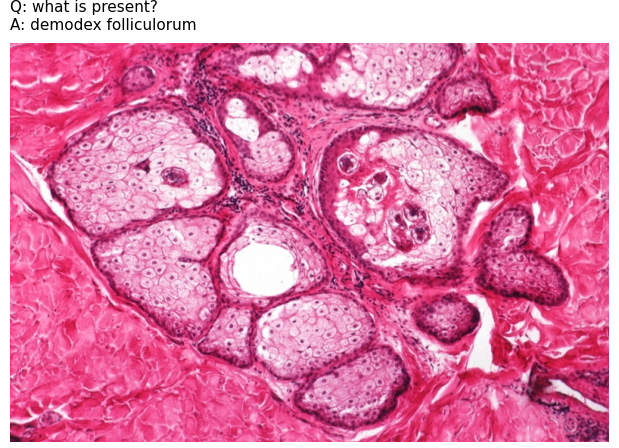
\includegraphics[width=2.45cm, height=1.55cm, keepaspectratio, trim=0 30 0 38, clip]{Images/vqa_method_sample.png}};
\node[tiny, align=left, anchor=north west] at ([xshift=0.18cm,yshift=-3.04cm]data.north west) {Answer: demodex folliculorum};
\node[flowbox, minimum width=2.35cm, minimum height=0.58cm] (prompt) at (0,-3.12) {\scriptsize Prompt control};

\node[groupbox, minimum width=3.25cm, minimum height=4.75cm, right=0.75cm of data] (models) {};
\node[title] at ([yshift=-0.28cm]models.north) {Multimodal VLMs};
\node[childbox, minimum width=2.75cm] (qwen) at ([yshift=-1.18cm]models.north) {\scriptsize Qwen2.5-VL-3B-Instruct};
\node[childbox, minimum width=2.75cm] (llava) at ([yshift=-2.20cm]models.north) {\scriptsize LLaVA-1.5-7B};
\node[childbox, minimum width=2.75cm] (medgemma) at ([yshift=-3.22cm]models.north) {\scriptsize MedGemma-4B-it};

\node[groupbox, minimum width=3.15cm, minimum height=3.55cm, right=0.82cm of models] (generation) {};
\node[title] at ([yshift=-0.28cm]generation.north) {Answer generation};
\node[childbox, minimum width=2.55cm] (greedy) at ([yshift=-1.28cm]generation.north) {\scriptsize Greedy answer};
\node[childbox, minimum width=2.55cm, minimum height=0.55cm] (sampled) at ([yshift=-2.25cm]generation.north) {\scriptsize $K$ sampled answers};

\node[groupbox, minimum width=3.75cm, minimum height=1.60cm, right=0.85cm of generation.north east, anchor=north west, yshift=0.05cm] (quality) {};
\node[title] at ([yshift=-0.26cm]quality.north) {Answer quality};
\node[metricbox, minimum width=0.95cm] (bleu) at ([xshift=-1.20cm,yshift=-0.95cm]quality.north) {\scriptsize BLEU-1};
\node[metricbox, minimum width=0.95cm] (rouge) at ([yshift=-0.95cm]quality.north) {\scriptsize ROUGE-L};
\node[metricbox, minimum width=0.95cm] (meteor) at ([xshift=1.20cm,yshift=-0.95cm]quality.north) {\scriptsize METEOR};

\node[groupbox, minimum width=3.75cm, minimum height=2.55cm, right=0.85cm of generation.south east, anchor=north west, yshift=-0.05cm] (reliability) {};
\node[title] at ([yshift=-0.26cm]reliability.north) {Reliability analysis};
\node[metricbox, minimum width=1.18cm] (freq) at ([xshift=-1.15cm,yshift=-0.92cm]reliability.north) {\scriptsize AFD frequency};
\node[metricbox, minimum width=1.18cm] (semantic) at ([xshift=-1.15cm,yshift=-1.48cm]reliability.north) {\scriptsize Semantic AFD};
\node[metricbox, minimum width=1.18cm] (qa) at ([xshift=-1.15cm,yshift=-2.04cm]reliability.north) {\scriptsize Question-aligned uncertainty};
\node[flowbox, minimum width=1.15cm, minimum height=1.25cm] (detector) at ([xshift=1.12cm,yshift=-1.47cm]reliability.north) {\scriptsize AUROC\\[1pt]AUPRC\\[1pt]Risk--coverage};

\node[flowbox, minimum width=1.25cm, minimum height=0.50cm, right=0.82cm of quality.east, anchor=west, yshift=0.15cm] (accept) {\scriptsize Accept};
\node[flowbox, minimum width=1.25cm, minimum height=0.50cm, right=0.82cm of reliability.east, anchor=west, yshift=-0.15cm] (review) {\scriptsize Reject / review};
\node[tiny, align=center, right=0.38cm of $(accept.south east)!0.5!(review.north east)$, anchor=west] {rejection\\threshold};

\draw[arrow] (data.east) -- (models.west);
\draw[arrow] (prompt.east) -| ([yshift=-0.15cm]models.west);
\draw[arrow] (models.east) -- (generation.west);
\draw[arrow] (greedy.east) -| ([yshift=0.08cm]quality.west);
\draw[arrow] (sampled.east) -| ([yshift=-0.08cm]reliability.west);
\draw[arrow] (quality.east) -- (accept.west);
\draw[arrow] (reliability.east) -- (review.west);
\end{tikzpicture}
